\documentclass[14pt]{beamer}

\usetheme[subsectionpage=progressbar]{metropolis}
\setbeamertemplate{section in toc}[sections numbered]

\usepackage{tikz}
\usetikzlibrary{arrows.meta}
\usetikzlibrary{matrix}

\usepackage{multicol}
\usepackage[utf8]{inputenc}
\usepackage{xcolor}

% Indent the subsections in the toc a bit more
\setbeamertemplate{subsection in toc}
{\leavevmode\leftskip=3em\rlap{\hskip-2em$\quad$\inserttocsectionnumber.\inserttocsubsectionnumber}$\quad$\inserttocsubsection\par}

\title{Øvingsforelesning 8: Traversering av grafer}
\subtitle{TDT4120 Algoritmer og datastrukturer}

\date{22. oktober 2019}
\author{Fredrik Strupe}
\institute{NTNU}

\begin{document}

\maketitle
\begin{frame}
    \frametitle{Plan}
    \tableofcontents
\end{frame}

\section{Gjennomgang av øving 7}
\begin{frame}{First Frame}
    Hello, world!
\end{frame}

\section{Denne ukens pensum}
\begin{frame}[standout]
    Pensum: Kap. 22.1-22.4
\end{frame}

\subsection{Representasjon av grafer}
\begin{frame}{Representasjon av grafer}
    \centering

    \pause

    Gitt følgende graf:

    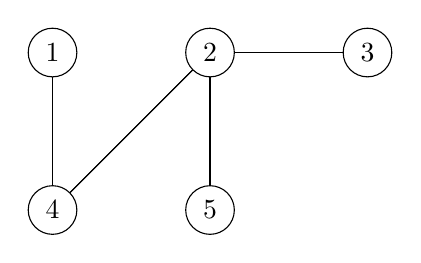
\begin{tikzpicture}
        \node[shape=circle,draw=black] (1) at (0,2) {1};
        \node[shape=circle,draw=black] (2) at (2,2) {2};
        \node[shape=circle,draw=black] (3) at (4,2) {3};
        \node[shape=circle,draw=black] (4) at (0,0) {4};
        \node[shape=circle,draw=black] (5) at (2,0) {5};

        \path [-] (1) edge node[left] {} (4);
        \path [-] (2) edge node[left] {} (3);
        \path [-] (2) edge node[left] {} (4);
        \path [-] (2) edge node[left] {} (5);
        \path [-] (3) edge node[left] {} (2);
        \path [-] (4) edge node[left] {} (1);
        \path [-] (4) edge node[left] {} (2);
        \path [-] (5) edge node[left] {} (2);
    \end{tikzpicture}

    \pause

    Hvordan kan vi representere grafen på en mer maskinvennlig måte?
\end{frame}
\begin{frame}{Representasjon av grafer}
    Hovedsakelig to måter:

    \begin{enumerate}
        \item<2->Som nabolister
        \item<3->Som nabomatrise
    \end{enumerate}
\end{frame}
\begin{frame}{Nabolister}
    \begin{columns}
        \column{0.5\textwidth}
            \begin{tikzpicture}
                \only<1>{\node[shape=circle,draw=black]} (1) at (0,2) {1};
                \only<2>{\node[shape=circle,draw=black,dashed]} (1) at (0,2) {1};
                \only<3->{\node[shape=circle,draw=black]} (1) at (0,2) {1};

                \only<-3>{\node[shape=circle,draw=black]} (2) at (2,2) {2};
                \only<4>{\node[shape=circle,draw=black,dashed]} (2) at (2,2) {2};
                \only<5->{\node[shape=circle,draw=black]} (2) at (2,2) {2};

                \only<-5>{\node[shape=circle,draw=black]} (3) at (4,2) {3};
                \only<6>{\node[shape=circle,draw=black,dashed]} (3) at (4,2) {3};
                \only<7->{\node[shape=circle,draw=black]} (3) at (4,2) {3};

                \only<-7>{\node[shape=circle,draw=black]} (4) at (0,0) {4};
                \only<8>{\node[shape=circle,draw=black,dashed]} (4) at (0,0) {4};
                \only<9->{\node[shape=circle,draw=black]} (4) at (0,0) {4};

                \only<-9>{\node[shape=circle,draw=black]} (5) at (2,0) {5};
                \only<10>{\node[shape=circle,draw=black,dashed]} (5) at (2,0) {5};
                \only<11->{\node[shape=circle,draw=black]} (5) at (2,0) {5};

                \path [-] (1) edge node[left] {} (4);
                \path [-] (2) edge node[left] {} (3);
                \path [-] (2) edge node[left] {} (4);
                \path [-] (2) edge node[left] {} (5);
                \path [-] (3) edge node[left] {} (2);
                \path [-] (4) edge node[left] {} (1);
                \path [-] (4) edge node[left] {} (2);
                \path [-] (5) edge node[left] {} (2);
            \end{tikzpicture}
        \column{0.5\textwidth}
            $1 \rightarrow \begin{bmatrix}\alt<3->{4}{~}\end{bmatrix}$\\
            $2 \rightarrow \begin{bmatrix}\alt<5->{3&4&5}{~}\end{bmatrix}$\\
            $3 \rightarrow \begin{bmatrix}\alt<7->{2}{~}\end{bmatrix}$\\
            $4 \rightarrow \begin{bmatrix}\alt<9->{1&2}{~}\end{bmatrix}$\\
            $5 \rightarrow \begin{bmatrix}\alt<11->{2}{~}\end{bmatrix}$\\
    \end{columns}
\end{frame}
\begin{frame}{Nabomatrise}
    \begin{columns}
        \column{0.5\textwidth}
            \begin{tikzpicture}
                \only<1>{\node[shape=circle,draw=black]} (1) at (0,2) {1};
                \only<2>{\node[shape=circle,draw=black,dashed]} (1) at (0,2) {1};
                \only<3->{\node[shape=circle,draw=black]} (1) at (0,2) {1};

                \only<-3>{\node[shape=circle,draw=black]} (2) at (2,2) {2};
                \only<4>{\node[shape=circle,draw=black,dashed]} (2) at (2,2) {2};
                \only<5->{\node[shape=circle,draw=black]} (2) at (2,2) {2};

                \only<-5>{\node[shape=circle,draw=black]} (3) at (4,2) {3};
                \only<6>{\node[shape=circle,draw=black,dashed]} (3) at (4,2) {3};
                \only<7->{\node[shape=circle,draw=black]} (3) at (4,2) {3};

                \only<-7>{\node[shape=circle,draw=black]} (4) at (0,0) {4};
                \only<8>{\node[shape=circle,draw=black,dashed]} (4) at (0,0) {4};
                \only<9->{\node[shape=circle,draw=black]} (4) at (0,0) {4};

                \only<-9>{\node[shape=circle,draw=black]} (5) at (2,0) {5};
                \only<10>{\node[shape=circle,draw=black,dashed]} (5) at (2,0) {5};
                \only<11->{\node[shape=circle,draw=black]} (5) at (2,0) {5};

                \path [-] (1) edge node[left] {} (4);
                \path [-] (2) edge node[left] {} (3);
                \path [-] (2) edge node[left] {} (4);
                \path [-] (2) edge node[left] {} (5);
                \path [-] (3) edge node[left] {} (2);
                \path [-] (4) edge node[left] {} (1);
                \path [-] (4) edge node[left] {} (2);
                \path [-] (5) edge node[left] {} (2);
            \end{tikzpicture}
        \column{0.5\textwidth}
            \begin{math}
                \begin{array}{c c} &
                \begin{array}{c c c c c} 1 & 2 & 3 & 4 & 5 \\
                \end{array}
                \\
                \begin{array}{c c c c c}
                1 \\ 2 \\ 3 \\ 4 \\ 5
                \end{array}
                &
                \left[
                \begin{array}{c c c c c}
                0 & 0 & 0 & \alt<3->{1}{0} & 0 \\
                0 & 0 & \alt<5->{1}{0} & \alt<5->{1}{0} & \alt<5->{1}{0} \\
                0 & \alt<5->{1}{0} & 0 & 0 & 0 \\
                \alt<3->{1}{0} & \alt<5->{1}{0} & 0 & 0 & 0 \\
                0 & \alt<5->{1}{0} & 0 & 0 & 0 \\
                \end{array}
                \right]
                \end{array}
            \end{math}
    \end{columns}
\end{frame}

\subsection{Bredde-først-søk}
\begin{frame}{Bredde-først-søk}
    Bredde-først-søk (BFS) er en algortime for å traversere grafer, som vil si å besøke noder i en viss rekkefølge.

    \pause

    Den "søker i bredden" ved å plassere noder i en kø, som den deretter velger fra.
\end{frame}
\begin{frame}{Bredde-først-søk}
    BFS fungerer omtrent slik:

    \begin{enumerate}
        \setcounter{enumi}{-1}
        \item<2-> Velg en startnode og legg denne inn i en kø.
        \item<3-> Hent ut noden som er fremst i køen.
        \item<4-> Legg til nodens naboer (som ikke allerede er besøkt eller i køen) bakerst i køen, og farg noden svart.
        \item<5-> Gjenta (gå til 1) til køen er tom.
    \end{enumerate}
\end{frame}
\begin{frame}{Bredde-først-søk}
    \begin{columns}
        \column{0.5\textwidth}
            \begin{tikzpicture}
                \only<-7>{\node[shape=circle,draw=black]} (1) at (0,2) {1};
                \only<8-10>{\node[shape=circle,draw=black,fill=lightgray]} (1) at (0,2) {1};
                \only<11>{\node[shape=circle,draw=black,fill=lightgray,dashed]} (1) at (0,2) {1};
                \only<12->{\node[shape=circle,draw=black,fill=black,text=white]} (1) at (0,2) {1};

                \only<-3>{\node[shape=circle,draw=black]} (2) at (2,2) {2};
                \only<4>{\node[shape=circle,draw=black,fill=lightgray]} (2) at (2,2) {2};
                \only<5>{\node[shape=circle,draw=black,fill=lightgray,dashed]} (2) at (2,2) {2};
                \only<6->{\node[shape=circle,draw=black,fill=black,text=white]} (2) at (2,2) {2};

                \only<1>{\node[shape=circle,draw=black]} (3) at (4,2) {3};
                \only<2>{\node[shape=circle,draw=black,fill=lightgray]} (3) at (4,2) {3};
                \only<3>{\node[shape=circle,draw=black,fill=lightgray,dashed]} (3) at (4,2) {3};
                \only<4->{\node[shape=circle,draw=black,fill=black,text=white]} (3) at (4,2) {3};

                \only<-5>{\node[shape=circle,draw=black]} (4) at (0,0) {4};
                \only<6>{\node[shape=circle,draw=black,fill=lightgray]} (4) at (0,0) {4};
                \only<7>{\node[shape=circle,draw=black,fill=lightgray,dashed]} (4) at (0,0) {4};
                \only<8->{\node[shape=circle,draw=black,fill=black,text=white]} (4) at (0,0) {4};

                \only<-5>{\node[shape=circle,draw=black]} (5) at (2,0) {5};
                \only<6-8>{\node[shape=circle,draw=black,fill=lightgray]} (5) at (2,0) {5};
                \only<9>{\node[shape=circle,draw=black,fill=lightgray,dashed]} (5) at (2,0) {5};
                \only<10->{\node[shape=circle,draw=black,fill=black,text=white]} (5) at (2,0) {5};

                \path [-] (1) edge node[left] {} (4);
                \path [-] (2) edge node[left] {} (3);
                \path [-] (2) edge node[left] {} (4);
                \path [-] (2) edge node[left] {} (5);
                \path [-] (3) edge node[left] {} (2);
                \path [-] (4) edge node[left] {} (1);
                \path [-] (4) edge node[left] {} (2);
                \path [-] (5) edge node[left] {} (2);
            \end{tikzpicture}
        \column{0.5\textwidth}
        Nodekø:
        \begin{math}
            \only<2>{3}
            \only<4>{2}
            \only<6>{4,5}
            \only<7>{5}
            \only<8>{5,1}
            \only<9-10>{1}
            \only<11->{}
        \end{math}

        Besøkt: $\only<3->{3} \only<5->{,2} \only<7->{,4} \only<9->{,5} \only<11->{,1}$

        Farget svart: $\only<4->{3} \only<6->{,2} \only<8->{,4} \only<10->{,5} \only<12->{, 1}$

        \begin{alertblock}
            \only<13->{Merk at besøkt = farget svart}
        \end{alertblock}

    \end{columns}
\end{frame}

\subsection{Dybde-først-søk}
\begin{frame}{Dybde-først-søk}
    Dybde-først-søk (DFS) er også en algoritme for graftraversering, og er relativt lik BFS.

    \pause

    I motsetning til BFS, kan DFS implementeres både iterativt og rekursivt.
\end{frame}
\begin{frame}{Dybde-først-søk}
    Den iterative implementasjonen er nesten helt lik BFS.

    \pause

    Hovedforskjellen er at DFS "søker i dybden" ved å alltid velge den \textit{bakerste} noden i køen, istedenfor den fremste.

    \pause

    Den bruker altså en stakk istedenfor en (LIFO-)kø.
\end{frame}
\begin{frame}{Dybde-først-søk}
    \textbf{OBS:} I pensumboka er kun den \textit{rekursive} implementasjonen beskrevet.

    \pause

    Vi kommer derfor til å fokusere på denne her.
\end{frame}
\begin{frame}{Dybde-først-søk}
    Rekursiv DFS fungerer omtrent slik:

%     \begin{enumerate}
%         \setcounter{enumi}{-1}
%         \item<2-> Velg en (vilkårlig) startnode.
%         \item<3-> Farg noden grå.
%         \item<4-> Legg til nodens ubesøkte naboer på toppen av stakken, og farg noden svart \textit{hvis ingen nye naboer ble lagt til i stakken}.
%         \item<5-> Gjenta (gå til 1) til stakken er tom.
%         \item<6-> Gjenta (gå til 0) til alle nodene er besøkt.
%     \end{enumerate}
\end{frame}
\begin{frame}{Dybde-først-søk}
    \begin{columns}
        \column{0.5\textwidth}
            \begin{tikzpicture}
                \only<-7>{\node[shape=circle,draw=black]} (1) at (0,2) {1};
                \only<8>{\node[shape=circle,draw=black,fill=lightgray]} (1) at (0,2) {1};
                \only<9>{\node[shape=circle,draw=black,fill=lightgray,dashed]} (1) at (0,2) {1};
                \only<10->{\node[shape=circle,draw=black,fill=black,text=white]} (1) at (0,2) {1};

                \only<-3>{\node[shape=circle,draw=black]} (2) at (2,2) {2};
                \only<4,6-12,14-16>{\node[shape=circle,draw=black,fill=lightgray]} (2) at (2,2) {2};
                \only<5,13,17>{\node[shape=circle,draw=black,fill=lightgray,dashed]} (2) at (2,2) {2};
                \only<18->{\node[shape=circle,draw=black,fill=black,text=white]} (2) at (2,2) {2};

                \only<1>{\node[shape=circle,draw=black]} (3) at (4,2) {3};
                \only<2,4-18>{\node[shape=circle,draw=black,fill=lightgray]} (3) at (4,2) {3};
                \only<3,19>{\node[shape=circle,draw=black,fill=lightgray,dashed]} (3) at (4,2) {3};
                \only<20->{\node[shape=circle,draw=black,fill=black,text=white]} (3) at (4,2) {3};

                \only<-5>{\node[shape=circle,draw=black]} (4) at (0,0) {4};
                \only<6,8-10>{\node[shape=circle,draw=black,fill=lightgray]} (4) at (0,0) {4};
                \only<7,11>{\node[shape=circle,draw=black,fill=lightgray,dashed]} (4) at (0,0) {4};
                \only<12->{\node[shape=circle,draw=black,fill=black,text=white]} (4) at (0,0) {4};

                \only<-5>{\node[shape=circle,draw=black]} (5) at (2,0) {5};
                \only<6-14>{\node[shape=circle,draw=black,fill=lightgray]} (5) at (2,0) {5};
                \only<15>{\node[shape=circle,draw=black,fill=lightgray,dashed]} (5) at (2,0) {5};
                \only<16->{\node[shape=circle,draw=black,fill=black,text=white]} (5) at (2,0) {5};

                \only<-20>{\node[shape=circle,draw=black]} (6) at (4,0) {6};
                \only<21>{\node[shape=circle,draw=black,fill=lightgray]} (6) at (4,0) {6};
                \only<22>{\node[shape=circle,draw=black,fill=lightgray,dashed]} (6) at (4,0) {6};
                \only<23->{\node[shape=circle,draw=black,fill=black,text=white]} (6) at (4,0) {6};

                \path [-] (1) edge node[left] {} (4);
                \path [-] (2) edge node[left] {} (3);
                \path [-] (2) edge node[left] {} (4);
                \path [-] (2) edge node[left] {} (5);
                \path [-] (3) edge node[left] {} (2);
                \path [-] (4) edge node[left] {} (1);
                \path [-] (4) edge node[left] {} (2);
                \path [-] (5) edge node[left] {} (2);
            \end{tikzpicture}
        \column{0.5\textwidth}
        Nodestakk:
        \begin{math}
            \only<2>{3}
            \only<4>{2}
            \only<6>{5,4}
            \only<7>{5}
            \only<8>{5,2,1}
            \only<9>{5,2,4}
            \only<11->{}
        \end{math}

        Besøkt: $\only<3->{3} \only<5->{,2} \only<7->{,4} \only<9->{,5} \only<11->{,1}$

        Farget svart: $\only<4->{3} \only<6->{,2} \only<8->{,4} \only<10->{,5} \only<12->{, 1}$

        \begin{alertblock}
            \only<13->{Merk at besøkt = farget svart}
        \end{alertblock}

    \end{columns}
\end{frame}
\begin{frame}
    Noe med kantklassifisering
\end{frame}


\subsection{Topologisk sortering}
\begin{frame}{Topologisk sortering}
    Topologisk sortering er en måte å ordne/sortere noder i en graf på.

    \pause

    Grafen må være rettet og asyklisk (en \textit{DAG}).

    \pause

    Vi får en topologisk sortering ved å kjøre DFS på grafen og sortere etter når noden ble farget svart.
\end{frame}
\begin{frame}{Topologisk sortering}
    \textbf{Men ...}

    \pause

    ... vi trenger ikke kjøre DFS hvis vi bare skal sjekke om en topologisk sortering er korrekt!

    \pause

    For en gyldig topologisk sortering vil alle nodene ha kanter som går mot høyre.
\end{frame}
\begin{frame}{Topologisk sortering}
    \begin{columns}
        \column{0.5\textwidth}
            \begin{tikzpicture}
                \node[shape=circle,draw=black] (1) at (0,2) {1};
                \node[shape=circle,draw=black] (2) at (2,2) {2};
                \node[shape=circle,draw=black] (3) at (4,2) {3};
                \node[shape=circle,draw=black] (4) at (0,0) {4};
                \node[shape=circle,draw=black] (5) at (2,0) {5};
                \node[shape=circle,draw=black] (6) at (4,0) {6};

                \path [-{Latex[length=3mm]},width=2] (2) edge node[left] {} (3);
                \path [-{Latex[length=3mm]},width=2] (2) edge node[left] {} (4);
                \path [-{Latex[length=3mm]},width=2] (4) edge node[left] {} (1);
                \path [-{Latex[length=3mm]},width=2] (5) edge node[left] {} (2);
            \end{tikzpicture}
        \column{0.5\textwidth}
            \onslide<2->{Er $1, 2, 3, 4, 5, 6$ en gyldig topologisk sortering?}

            \onslide<5->{\textcolor{red}{Nei!}}
    \end{columns}
    \vfill
    \centering
    \onslide<3->{
        \begin{tikzpicture}
            \node[shape=circle,draw=black] (1) at (0,0) {1};
            \node[shape=circle,draw=black] (2) at (2,0) {2};
            \node[shape=circle,draw=black] (3) at (4,0) {3};
            \node[shape=circle,draw=black] (4) at (6,0) {4};
            \node[shape=circle,draw=black] (5) at (8,0) {5};
            \node[shape=circle,draw=black] (6) at (10,0) {6};

            \onslide<4->{
                \path[-{Latex[length=3mm]},width=2] (2) edge[bend left] node[left] {} (3);
                \path[-{Latex[length=3mm]},width=2] (2) edge[bend left] node[left] {} (4);
                \path[-{Latex[length=3mm]},width=2] (4) edge[bend right] node[left] {} (1);
                \path<5->[-{Latex[length=3mm]},width=2,color=red] (4) edge[bend right] node[left] {} (1);
                \path[-{Latex[length=3mm]},width=2] (5) edge[bend left] node[left] {} (2);
                \path<5->[-{Latex[length=3mm]},width=2,color=red] (5) edge[bend left] node[left] {} (2);
            }
        \end{tikzpicture}
    }
\end{frame}
\begin{frame}{Topologisk sortering}
    \begin{columns}
        \column{0.5\textwidth}
            \begin{tikzpicture}
                \node[shape=circle,draw=black] (1) at (0,2) {1};
                \node[shape=circle,draw=black] (2) at (2,2) {2};
                \node[shape=circle,draw=black] (3) at (4,2) {3};
                \node[shape=circle,draw=black] (4) at (0,0) {4};
                \node[shape=circle,draw=black] (5) at (2,0) {5};
                \node[shape=circle,draw=black] (6) at (4,0) {6};

                \path [-{Latex[length=3mm]},width=2] (2) edge node[left] {} (3);
                \path [-{Latex[length=3mm]},width=2] (2) edge node[left] {} (4);
                \path [-{Latex[length=3mm]},width=2] (4) edge node[left] {} (1);
                \path [-{Latex[length=3mm]},width=2] (5) edge node[left] {} (2);
            \end{tikzpicture}
        \column{0.5\textwidth}
            \onslide<2->{Er $6, 5, 2, 3, 4, 1$ en gyldig topologisk sortering?}

            \onslide<5->{\textcolor{green}{Ja!}}
    \end{columns}
    \vfill
    \centering
    \onslide<3->{
        \begin{tikzpicture}
            \node[shape=circle,draw=black] (6) at (0,0) {6};
            \node[shape=circle,draw=black] (5) at (2,0) {5};
            \node[shape=circle,draw=black] (2) at (4,0) {2};
            \node[shape=circle,draw=black] (3) at (6,0) {3};
            \node[shape=circle,draw=black] (4) at (8,0) {4};
            \node[shape=circle,draw=black] (1) at (10,0) {1};

            \onslide<4->{
                \path[-{Latex[length=3mm]},width=2] (2) edge[bend right] node[left] {} (3);
                \path[-{Latex[length=3mm]},width=2] (2) edge[bend left] node[left] {} (4);
                \path[-{Latex[length=3mm]},width=2] (4) edge[bend right] node[left] {} (1);
                \path[-{Latex[length=3mm]},width=2] (5) edge[bend left] node[left] {} (2);
            }
        \end{tikzpicture}
    }
\end{frame}



\section{Tips til øving 8, teori}
\begin{frame}{Tips 1}
    I denne forelesningen gikk vi gjennom BFS og DFS på urettede grafer.

    \pause

    De fungerer helt likt med rettede grafer!
\end{frame}
\begin{frame}{Tips 2}
    Kompleksitene som bes om i teoriøvingen finnes i pensumboka og/eller på nettet ...

    \pause

    ... men prøv å forstå hvorfor de er som de er.
\end{frame}
\begin{frame}{Tips 3}
    BFS- og DFS-øvingene spør om hvilken rekkefølge nodene blir \textit{farget svar}.

    \pause

    Ikke i hvilken rekkefølge de først ble besøkt!
\end{frame}
\begin{frame}{Tips 4}
    Kantklassifisering i DFS kan være litt tricky ...

    \pause

    ... men bruk eliminasjonsmetoden.
\end{frame}

\section{Tips til øving 8, praksis}
\begin{frame}[fragile]{Oppgave 1}
    Oppgaven er å implementere \verb|mazetonodelist(maze)|.

    \pause

    Det står allerede en del info i oppgaven, men her kommer enda et eksempel.
\end{frame}
\begin{frame}[fragile]{Oppgave 1}
    \verb|maze = |
    \vfill

    \alt<2->{\colorlet{cl1}{gray}}{\colorlet{cl1}{block body.bg}}

    \begin{center}
    \begin{tikzpicture}
    \matrix [matrix of nodes,row sep=-\pgflinewidth]
    {
        ~ & \textcolor{cl1}{1} & \textcolor{cl1}{2} & \textcolor{cl1}{3} & \textcolor{cl1}{4} & \textcolor{cl1}{5} & \textcolor{cl1}{6} & \textcolor{cl1}{7} \\
        \textcolor{cl1}{1} & 0 & 0 & 0 & 0 & 0 & 0 & 0 \\
        \textcolor{cl1}{2} & 1 & 1 & 0 & 1 & 1 & 1 & 0 \\
        \textcolor{cl1}{3} & 0 & 1 & 0 & 1 & 0 & 0 & 0 \\
        \textcolor{cl1}{4} & 0 & 1 & 0 & 1 & 1 & 1 & 0 \\
        \textcolor{cl1}{5} & 0 & 1 & 1 & 1 & 0 & 1 & 0 \\
        \textcolor{cl1}{6} & 0 & 1 & 0 & 1 & 0 & 1 & 1 \\
        \textcolor{cl1}{7} & 0 & 0 & 0 & 0 & 0 & 0 & 0 \\
    };
    \end{tikzpicture}
    \end{center}
\end{frame}
\begin{frame}[fragile]{Oppgave 1}
    \verb|maze = |
    \vfill

    \colorlet{cl1}{gray}

    \begin{center}
    \begin{tikzpicture}
    \matrix [matrix of nodes,row sep=-\pgflinewidth]
    {
        ~ & \textcolor{cl1}{1} & \textcolor{cl1}{2} & \textcolor{cl1}{3} & \textcolor{cl1}{4} & \textcolor{cl1}{5} & \textcolor{cl1}{6} & \textcolor{cl1}{7} \\
        \textcolor{cl1}{1} & \node[shape=circle,draw=black] (1) {1}; & \node[shape=circle,draw=black] (1) {1}; & 0 & 0 & 0 & 0 & 0 \\
        \textcolor{cl1}{2} & 1 & 1 & 0 & 1 & 1 & 1 & 0 \\
        \textcolor{cl1}{3} & 0 & 1 & 0 & 1 & 0 & 0 & 0 \\
        \textcolor{cl1}{4} & 0 & 1 & 0 & 1 & 1 & 1 & 0 \\
        \textcolor{cl1}{5} & 0 & 1 & 1 & 1 & 0 & 1 & 0 \\
        \textcolor{cl1}{6} & 0 & 1 & 0 & 1 & 0 & 1 & 1 \\
        \textcolor{cl1}{7} & 0 & 0 & 0 & 0 & 0 & 0 & 0 \\
    };
    \end{tikzpicture}
    \end{center}
\end{frame}

\begin{frame}{bleh}
\end{frame}
\end{document}
